\documentclass[abstract=on,10pt,a4paper,bibliography=totocnumbered]{article}
\usepackage[paper=a4paper,left=35mm,right=35mm,top=25mm,bottom=30mm]{geometry}
\usepackage[doublespacing]{setspace}
\usepackage[english]{babel}
\usepackage[utf8]{inputenc}
\usepackage[round]{natbib}
\usepackage{amsmath}
\usepackage{colortbl}
\usepackage{amsfonts}
\usepackage{amssymb}
\usepackage{gensymb}
\usepackage{graphicx}
\usepackage{tikz}
\usepackage{enumerate}
\usepackage{enumitem}
\usepackage{subcaption}
\usepackage{booktabs}
\usepackage[hidelinks]{hyperref}
\usepackage[nameinlink]{cleveref}
% \usepackage{lineno}
\usepackage{multirow}
\usepackage{arydshln}
% \usepackage[nomarkers, nolists]{endfloat}

%------------------------------------------------------------------------------
%	Some Styling
%------------------------------------------------------------------------------
% Creating some TikZ styles
\tikzset{
  nonterminal/.style = {rectangle
    , minimum size = 6mm
    , very thick
    , draw = black!
  }
}

% Changing the style of captions in figures etc.
\captionsetup{labelfont=bf, format=plain, font=small}

% Change how equations are referenced
\renewcommand{\theequation}{Equation \arabic{equation}}%

%------------------------------------------------------------------------------
%	Titlepage: Header
%------------------------------------------------------------------------------
\title{Step by Step: Using Integrated Step Selection Analysis to Simulate Wild
Dog Dispersal and Assess Landscape Connectivity}

% List of Authors
\author{
  David D. Hofmann\textsuperscript{1,\S} \and
  John W. McNutt\textsuperscript{2} \and
  Arpat Ozgul\textsuperscript{1} \and
  Gabriele Cozzi\textsuperscript{1,2} \and
  Dominik M. Behr\textsuperscript{1,2}
}

% Reduce spacing between authors
\makeatletter
\def\and{%
  \end{tabular}%
  \hskip -0.5em \@plus.17fil\relax
  \begin{tabular}[t]{c}}
\makeatother

% Current Date
\date{\today}

% And here the masterpiece begins
\begin{document}

% Change page numbering
\pagenumbering{gobble}

% Required to be able to cite
\bibliographystyle{apalike}

% Create Titlepage
\maketitle

%------------------------------------------------------------------------------
%	Titlepage: Additional Info
%------------------------------------------------------------------------------
\begin{flushleft}

\vspace{0.5cm}

\textsuperscript{1} Department of Evolutionary Biology and Environmental
Studies, University of Zurich, Winterthurerstarsse 190, 8057 Zurich,
Switzerland.

\textsuperscript{2} Botswana Predator Conservation Trust, Private Bag 13, Maun,
Botswana.

\textsuperscript{\S} Corresponding author (david.hofmann2@uzh.ch)

\vspace{4cm}

\textbf{Running Title:} Simulating Wild Dog Dispersal.

\vspace{0.5cm}

\textbf{Keywords:} dispersal, habitat selection, integrated step selection
function, Kavango-Zambezi Transfrontier Conservation Area, landscape
connectivity, least-cost corridors, Lycaon pictus, permeability surface,
protected areas, wildlife management

\end{flushleft}

%------------------------------------------------------------------------------
%	Abstract
%------------------------------------------------------------------------------
\newpage
\begin{abstract}
This is the abstract.
\end{abstract}

%------------------------------------------------------------------------------
%	Main Text
%------------------------------------------------------------------------------
\newpage

% Change page numbering
\pagenumbering{arabic}

% % Create linenumbers
% \linenumbers

\section{Introduction}
An animals movement trajectory can be seen as the result of an interplay between
habitat and movement preferences.

In recent decades, least-cost analysis has become the workhorse to study
landscape connectivty at large scales. Originally introduced by XX, the concept
and relating methods have been refined to more realistically render animal's
movement capabilities and to determine valuable movement corridors that require
protection. (talk a bit about different methods of LCPs, see methods in
gdistance package). More recently, more attention has been assigned to the
collection of movement data is better tailored towards assessing landscape
connectivity. In particular, it has been proposed and verified that relocation
data collected dispersing individuals leads to more accurate and reliable
estimates of landscape connectivity. This superiority of dispersal data in
comparison to data that stem from residents is mainly owed to the fact that
animals behave vastly different during residency. Despite substantial advances
in ecologists ability to track animals in space and time, dispersal remains one
of the most difficult behavioral modes to observe in wild animals. Especially
for wide ranging and long-lived species, dispersal is difficult to predict and
observe, such that data remains scarce.

Many connectivity modelling techniques, especially least-cost analysis,
implicitly assume that the studied animal has partial or even complete knowledge
of the landscape and associated movement costs. While this assumption may be
reasonable for migrating animals that move between a limited number of habitats,
yet it is unlikely to hold for dispersers. In contrast to migrants, dispersers
move into unknown territory and are therefore confronted with novel landscapes.
Consequently, dispersers are more likely to adjust their movement behavior
\textit{ad hoc} instead of preplanning an entire trajectory. As a result,
methods that assume complete knowledge of the landscape and subsequent optimal
movement behavior likely misrepresent true dispersal behavior. As such, methods
that allow a more random approach to a dispersers movement behavior may more
realistically render the movement corridors of dispersing individuals.

In addition, individual based simulations will allow to explicitly model
dispersal between subpopulations in models of population dynamics.

Reliable identification of dispersal corridors will become increasingly
important with the uprise of ever-growing and often transboundary conservation
areas. One such instance is the KAZA-TFCA, a massive conservation area spanning
five countries and over 520'000 km\textsuperscript{2}. The KAZA holds the
potential of re-establishing dispersal routes for many of its protected species,
including the african wild dog \textit{Lycaon pictus}. This species has
experienced severe population declines caused by human induced mortality and
deadly diseases. In result, the species currently marks the KAZA's most
endangered large carnivore and has been a assigned a very high conservation
priority. Importantly, due to their inherent mobility and intrinsic need for
vast undisturbed landscapes, AWDs have been proposed as surrogate species for
landscape connectivity (see recent paper on multispecies connectivity).
Nevertheless, the species has received little attention in the connectivity
literature, mainly due to the difficulty in observing wild dog dispersal. In a
previous paper, we addressed this issue and developed a habitat selection model
based on which we predicted landscape connectivity using least-cost corridor
analysis. We now expand on this knowledge and develop a more detailed movement
model of dispersing wild dogs. We then use this model to simulate thousands of
dispersers moving throughout the KAZA. Based on said simulations, we compute
heatmaps and identify potential dispersal hotspots and compare them to the
dispersal routes identified in (Hofmann ....). We also apply the data to feed a
network-analysis, based on which we determine network-metrics pertinent to
landscape connectivity.

\section{Methods}
\subsection{Study Area}
The study area (centered at -17\degree 13'9''S, 23\degree 56'4''E;
\Cref{StudyArea}a) stretched over 1.3 Mio km\textsuperscript{2} and ecompassed
the entire KAZA-TFCA (\Cref{StudyArea}b). The KAZA-TFCA is the world's largest
transboundary conservation area and comprises parts of Angola, Botswana,
Namibia, Zimbabwe, and Zambia, covering a total area of over 520'000
km\textsuperscript{2}. Its landscape varies regionally and ranges from savanna,
to grassland, and from dry to moist woodland habitats. A dominant
hydrogeographical feature in its center is the Okavango Delta, the earth's
largest inland delta and home to a vast diversity of mammal species. The delta
and its surroundings are considered a stronghold for African wild dogs which may
act as a source for the recolonization of surrounding habitats. The wet season
in the region lasts from November to March, albeit the main floodwaters reach
the Delta between July and August after descending through the Angolian
highlands \citep{McNutt.1996, Wolski.2017}.

\begin{figure}[htbp]
  \begin{center}
    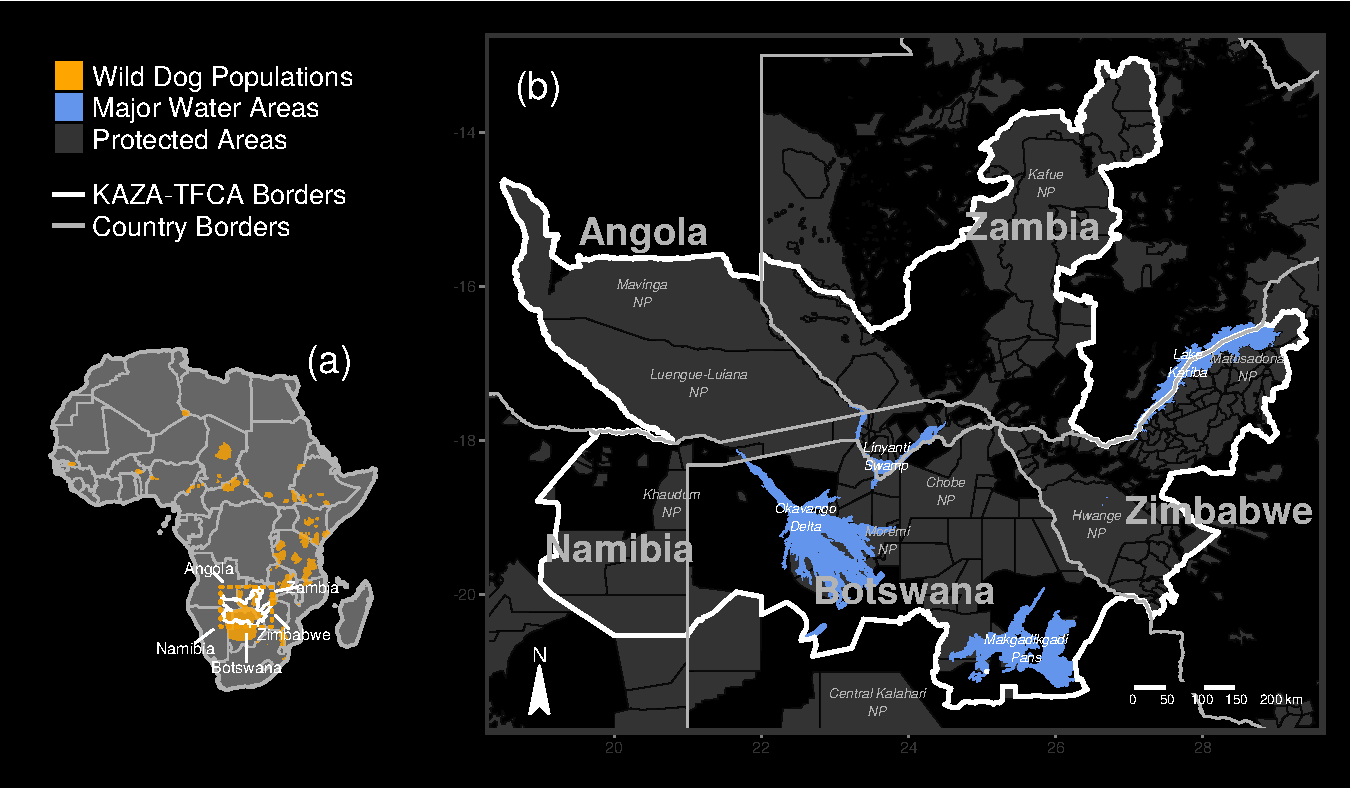
\includegraphics[width = \textwidth]{99_StudyArea}
    \caption{Study area}
    \label{StudyArea}
  \end{center}
\end{figure}

\subsection{GPS Relocation Data}
Between 2011 and 2020, we collected GPS relocation data on free-ranging wild
dogs inhabiting the Okavango Delta in northern Botswana. We identified potential
dispersers based on criteria reported in \cite{Behr.2020}, immobilized them
according to protocols described in \cite{Osofsky.1996}, and fitted them with
GPS/Satellite radio collars (\textit{Vertex Lite; Vectronic Aerospace GmbH,
Berlin}). Handling and collaring of all individuals was carried out and
supervised by a Botswana-registered wildlife veterinarian. Of all collared
individuals, a total of 16 individuals dispersed, each in a same-sex coalition
(7 female and 9 male coalitions). When we observed dispersal we remotely
increased the GPS fixrate from 24 to 4 hours. Collected relocations were then
regularly transmitted via Iridium satellite system to a base station. This
allowed remote tracking of dispersers even if they left the main study area or
crossed international borders. To effectively distinguish between resident and
dispersersing individuals, we applied the net-squared displacement metric. This
metric measures the Euclidean distance of a collared individual to a reference
point \citep{Borger.2012}. In our case, these reference points resembled the
center of the dispersing coalition's natal home range. Hence, dispersal was
deemed to have started when an individual left its natal home range and ended
when the individual became stationary again. Previous research found no
differences between males and females during dispersal \citep{Woodroffe.2019,
Cozzi.2020}, so we did not distinguish sexes in our analyses. GPS relocations
were then converted to steps, where a step represented the straight-line
distance travelled between two consequtive GPS relocations
\citep{Turching.1998}.

\subsection{Covariates}
To represent environmental covariates spatially, we prepared a set of raster
layers depicting water-cover (dynamically updated), square rooted distance to
water (dynamically updated), tree-cover, and shrub/grassland-cover. We also
created a proxy for human influence, rendering anthropogenic pressures stemming
from human-density, agricultural sites, and roads. We prepared all layers at a
resolution of 250m by 250m for the extent of the entire KAZA-TFCA. A more
detailed description of the derivation and preparation of each environmental
covariate is given in \cite{Hofmann.2020}. Because wild dogs follow a diurnal
activity pattern, we coded a binary variable indicating whether an observed step
started during phases of main wild dog activity (07:00 a.m. and 07:00 p.m.) or
low wild dog activity (anything else).

\subsection{Movement Model}
We used integrated step selection functions (iSSF) to parametrize a mechanistic
movement model of dispersing wild dogs. In the iSSF framework, observed steps
receive a selection score \(w(x)\) that depends on the covariates \(X\)
experienced along a step, as well as the animals preferences towards these
covariates \(\beta\). In contrast to regular step selection analysis,
\textit{integrated} step selection analysis allows simulatneous inference on
movement and habitat preferences of the studied animal. Moreover, potential
interactions between habitat and movement preferences can be modelled. Thus, the
method produces more accurate selection estimates and allows to use the
resulting models as proper mechanistic movement models from which movement can
be generated. To conduct iSSf analysis, we paired each observed step with 24
random steps. Random steps basically resembled potential alternatives that the
animal could have realized but decided not to. We generated random steps by
sampling random turning angles from a uniform distribution (\(-\pi, +\pi\)) and
step lengths from a gamma distirbution that was fitted to observed steps (scale
= 6308, shape = 0.37). While the number of random steps is inversely
proportional to the sampling error \citep{Avgar.2016}, we found only minor
changes in inference when sampling further random steps. Along each step we
extracted spatial covariates using the \textit{velox} package. We also
calculated step metrics, namely the natural logarithm of the step length
\(log(sl\_\)) and the cosine of the turning angle \(cos(ta\_)\). We scaled all
continuous covariates to a mean of zero and a standard deviation of one. We then
used the r-package \textit{glmmTMB} to fit mixed effects conditional logistic
regression models as proposed by \citep{Muff.2020}. Our movement model was built
around a previously published habitat selection model of dispersing wild dogs.
Because the earlier model was used to predict landscape permeability,
interactions between environmental and spatial covariates were impossible to
model. Our current movement model, in contrast, allowed the inclusion of
additional interactions that describe differences in movement behavior induced
through different environments. Hence, we started with the habitat model and
iteratively increased model complexity by including additional interactions
between movement metrics and environmental covariates. That is, we proposed all
two-way interactions between spatial covariates and movement metrics. For
instance, for the covariate \textit{water} we proposed the interactions
Water:cos(ta\_) and Water:log(sl\_). Despite interactions between environmental
factors and movement metrics, we also proposed the interaction
\(log(sl\_):MainActivity\) to account for the diurnal activity pattern of wild
dogs. A preliminary revealed little differences in turning angles during main
and low activity, hence we did not include the interaction
\(cos(ta\_):MainActivity\). We then ran stepwise modal forward selection absed
on Akaike's Information Criterion (AIC, \citealp{Burnham.2002}) values and
identified the most parsimonious movement model.

\subsection{Dispersal Simulation}
We used the most parsimonious movement model to simulate dispersing wild dogs
departing from predefined source points. The simulation basically resembled an
inverted iSSF function and was set up as follows. First, we determined a source
point at which a disperser was initiated. To allow calculation of turning
angles, we assumed a random initial orientation of the animal. Second, we
proposed 25 random steps originating at the predefined source point. We
generated random steps by sampling turning angles from a uniform distribution
(\(-\pi, +\pi\)) and step lengths from a gamma distribution fitted to observed
step lengths. To prevent unrealistically large steps, we capped the gamma
distribution 35km, the farthest distance travelled in four hours according to
our data. Third, along each random step we extracted environmental covariates
calculated step metrics. Fourth, we applied the parametrized dispersal model to
predict selection scores \(w(x)\) and to determine the probability of a step
being realized. Fifth, we sampled one of the proposed based on their
probabilities and calculated the animal's new position. We then repeated steps
two to five until 2000 steps were realized. In case a proposed random step left
our study extent, we removed the step from the set of random steps, thereby
forcing the disperser to stay within the boundaries of the study area.

\subsection{Source Points}
Simulations from step selection functions are known to be sensitive to the
location of source points, which is why we followed a twofold approach to sample
release points across the KAZA-TFCA. In a first approach, we used the same 68
source points between which we already computed least-cost paths and least-cost
corridors (see xx). These source points were regularly spaced 100 km apart,
located within protected areas (\(>\) 700 km\textsuperscript{2}). Because of
the regulary spacing, not all protected areas received source points. Hence, we
placed additional source points at the center of such protected areas. At each
of the generated source point we released 1000 dispersers, implying a total of
68'000 simulated dispersers. In a second approach, we used the same 68 source
points to define catchment areas inside protected areas. That is, for each of
the 68 source points we defined its voronoi polygon within the point's protected
area. Within these catchment areas we then randomly sampled 1000 new source
points from which we released another 68'000 dispersers. Overall, we simulated
134'000 dispersers for a total of 268 Mio. steps.

\begin{figure}[htbp]
  \begin{center}
    \includegraphics[width = \textwidth]{99_SourcePoints}
    \caption{Illustration of source points from which dispersal was simulated.
    Although in reality we simulated 1'000 per source point, we illustrate an
    example assuming 10 dispersers from each source point. (a) Static source
    points similar to the source points reported in ... (b) Source points that
    were randomized within the catchment areas (dark gray, delinated by solid
    black lines).}
    \label{SourcePoints}
  \end{center}
\end{figure}

\subsection{Heatmaps}
Using the simulated trajectories we created heatmaps to examine through which
areas most simulated individuals dispersed. We rasterized all trajectories and
calculated how often each raster-cell was traversed by simulated dispersers. If
the same trajectory crossed a pixel twice, it was only counted once. We achieved
high performance rasterization of spatial lines using the recently developed
R-package \textit{terra} \citep{Hijmans.2020}. To examine if and how ``heat''
changes in response to changes in the location of source points and the number
of simulated steps, we followed a 2 x 6 design and created heatmaps for both
point sampling regines, as well as for 68, 125, 250, 500, 1000, and 2000
dispersal steps. We quantified the similarity of the resulting 12 heatmaps to
the permeability and least-cost corridor maps presented in (Hofmann ...) we used
Bhattacharyya's affinity. Bhattacharyya's affinity ranges from zero (complete
separation) to one (perfect match) and has earlier been proposed to compare the
overlap of utilisation distributions (Fieberg).

\subsection{Network Analysis I: Areas Reached}
Based on the simulated trajectories we identified to which other areas each
source area is connected. For instance, if a trajectory originated at source
point one and intersected with source areas two and three, we assumed that
source areas two and three were within reach of source are one. To get a sense
of the strength of connections, we also calculated how often each of these
connections was realized. This procedure resulted in 6 x 2 edge lists which we
further used to generate weighted networks and to calculate network metrics.

\subsection{Network Analysis II: Betweenness}
We coerced all simulated trajectories into a network consisting of vertices
(relocations) and edges (connections between relocations). To do so, we created
raster layers at multiple resolutions and identified each trajectory's
transition matrix on these rasters see figure xx \citep{Bastille.2018}. We then
merged the transition matrices of all trajectories and calculated cumulative
transitions between all raster-cells. This resulted in an edge-list, containing
all observed from-to connections as well as their frequency. Using this
edge-list, we generated a weighted graph using the r-package \textit{igraph}.
Based on this graph we calculated betweenness scores as well as the degree of
each raster cell. Betweenness indicates how often a specific raster-cell lies on
a shortest path between two other raster-cells and is a useful metric to detect
movement corridors. Degree, on the other hand, indicates how many connections a
raster cell has and therefore serves to illustrate the xxx of specific nodes.
When calculating betweenness, we used the transition frequency as weighting
factor. That is, a higher transition frequency contributed to a higher
betweenness score.

\subsection{Network Analysis III: Transitions}



\section{Results}
Compared to the base model, the most parsimonious movement model included
several additional interactions (\Cref{MovementModel} and Table S1). The model
indicates that dispersers move directional, particularly when distant to water,
yet less so in human dominated landscapes. Furthermore, dispersers prefer large
steps, especially during main activity. In contrast, step lengths tend to be
shorter when water- or tree-cover is high. In general, dispersers avoid water,
prefer proximity to water, avoid dense tree-cover, prefer shrubs/grassland, and,
finally, avoid human dominated landscapes.

\begin{figure}
  \begin{center}
    \begin{subfigure}[c]{0.8\textwidth}
      \includegraphics[width=\textwidth]{99_MovementModel}
      % \subcaption{Subfigure Bild Nr. 1}
    \end{subfigure}
    % \begin{subfigure}[c]{\textwidth}
    %   \includegraphics[width=\textwidth]{99_MovementModel(Interactions)}
    %   % \subcaption{Subfigure Bild Nr. 2}
    % \end{subfigure}
    \caption{Most parsimonious movement model. Whiskers delineate the 95\%
    Confidence-Intervals. Significance codes: * \(p < 0.10\), ** \(p < 0.05\),
    *** \(p < 0.01\).}
    \label{MovementModel}
  \end{center}
\end{figure}

\subsection{Heatmaps}
Six of the twelve rasterized dispersal trajectories are presented as heatmaps in
\Cref{Heatmaps}. As can be seen, differences that stem from the method of point
sampling disappear as more steps are simulated. This is to be expected as the
influence of the origin becomes smaller and smaller as the animal moves through
the landscape. However, there are striking differences when simualtions are only
run for few iterations.

\begin{figure}
  \includegraphics[width=\textwidth]{99_Heatmaps}
  \caption{}
  \label{Heatmaps}
\end{figure}

Bhattacharyya's affinity index supports the notion that heatmaps become more
similar to the earlier developed permeability and corridor maps as the number of
simulated steps increases. Furthermore, it appears that randomly sampled source
points contribute to a higher similarity too, albeit differences due to the
sampling regime vanish as the number of simulated steps increases. In fact, both
maps are almost identical to each other after 2000 steps. Furthermore, the
connectivity networks become increasingly similar to the previously published
permeability and corridor maps. Still, some differences remain even after 2000
simulated steps, highlighting that some severe impediments in the landscape
exist.

\begin{table}[hbtp]
  \caption{Summary statistics of all GPS relocations that have been recorded on
  dispersing coalitions.}
  \label{GPSData}
  \begin{center}
  \resizebox{\textwidth}{!}{
    \begin{tabular}{lllllllll}
    \toprule
    sampling & Metric & Map & 68 & 125 & 250 & 500 & 1000 & 2000 \\
    \midrule
    Static & Affinity & Corr & 0.64 & 0.70 & 0.76 & 0.80 & 0.82 & 0.84 \\
    Static & Affinity & Perm & 0.67 & 0.74 & 0.80 & 0.85 & 0.89 & 0.91 \\
    Static & Correlation & Corr & 0.32 & 0.38 & 0.45 & 0.51 & 0.56 & 0.60 \\
    Static & Correlation & Perm & 0.47 & 0.57 & 0.66 & 0.72 & 0.78 & 0.82 \\
    \hdashline
    Random & Affinity & Corr & 0.70 & 0.75 & 0.79 & 0.82 & 0.84 & 0.85 \\
    Random & Affinity & Perm & 0.74 & 0.79 & 0.83 & 0.87 & 0.90 & 0.92 \\
    Random & Correlation & Corr & 0.38 & 0.43 & 0.48 & 0.53 & 0.57 & 0.61 \\
    Random & Correlation & Perm & 0.58 & 0.64 & 0.69 & 0.75 & 0.79 & 0.83 \\
    \hdashline
    n.a. & Affinity & Heat & 0.76 & 0.86 & 0.94 & 0.97 & 0.99 & 0.99 \\
    n.a. & Correlation & Heat & 0.90 & 0.94 & 0.97 & 0.98 & 0.99 & 1.00 \\
    \bottomrule
    \end{tabular}
  }
  \end{center}
\end{table}

\section{Discussion}
Our connectivity network further suggests that dispersers from the Okavango
Delta more likely disperse towards east than west. Indeed, only x out of our y
observed dispersers ever reached the western part of the delta. Only when the
flood retracts a small pathway between the city of Maun and the floodwaters of
the delta emerges and enables dispersers to move towards the detal's western
part.

Our work suggests that the selection of source points significantly impacts
resulting connectivity networks. Especially when dispersal durations are short,
wrongly placed source points lead to vastly different results. Signer et al.
used estimated utilisation distributions by means of simulated movements. They
used a rather long burn in period prior to alleviate the problem of selecting
meaningful source points. However, this approach only works when individuals
move around a point of attraciton. This is typically not the case when
simulating dispersers, introducing an important trade-off. The researcher can
decide to increase the number of simulated steps, hence reducing the influence
of starting locations, yet this also inevitably increases estimated
connectivity.

\section{Authors' Contributions}
D.D.H., D.M.B., A.O. and G.C. conceived the study and designed methodology;
D.M.B., G.C., and J.W.M. collected the data; D.D.H. and D.M.B. analysed the
data; G.C. and A.O. assisted with modelling; D.D.H., D.M.B., and G.C. wrote the
first draft of the manuscript and all authors contributed to the drafts at
several stages and gave final approval for publication.

\section{Data Availability}
GPS movement data of dispersing coalitions will be made available on dryad at
the time of publication.

\section{Acknowledgements}
We thank the Ministry of Environment and Tourism of Botswana for granting
permission to conduct this research. We thank C. Botes, I. Clavadetscher, and G.
Camenisch for assisting with wild dog immobilizations. We also thank B. Abrahms
for sharing her data of three dispersing wild dogs. Furthermore, we are indebted
to Johannes Signer for assisting with the simulation algorithm. This study was
funded by Basler Stiftung für Biologische Forschung, Claraz Foundation, Idea
Wild, Jacot Foundation, National Geographic Society, Parrotia Stiftung, Stiftung
Temperatio, Wilderness Wildlife Trust Foundation, Forschungkredit der
Universität Zürich, and a Swiss National Science Foundation Grant
(31003A\_182286) to A. Ozgul.

\newpage
\begingroup
\singlespacing
\bibliography{Literatur}
\endgroup

\end{document}
